\section{Proposed method}
\label{sec:proposed-method}

The proposed protocol has three parts: a split that the case declares before any fit, a rule that fixes the training window of a case whose rows are dated, and three invariance gates, with a control that keeps them from passing vacuously, that are executed on the fitting path and must pass before a result is written. Figure~\ref{fig:protocol} shows the flow. The protocol is enforcement of rules that are already stated in the credit-scoring and machine-learning literature \citep{hastie2009,siddiqi2017,kaufman2012}; what is proposed is their formal statement, their per-case declaration, a test that fails when they are broken, and the measurement of what the test sees (Sections~\ref{sec:experimental-design} and~\ref{sec:results}).

\begin{figure}[htbp]
\centering
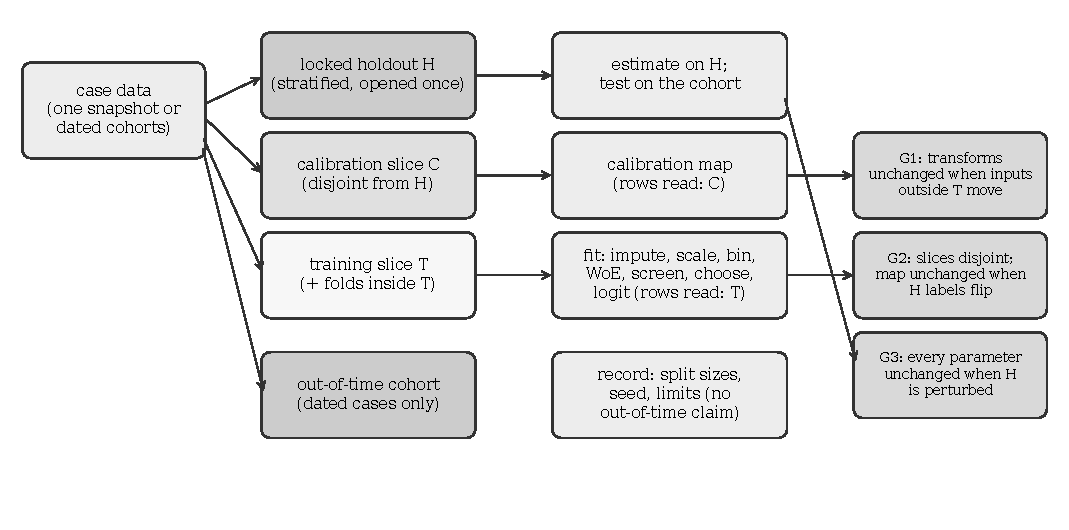
\includegraphics[width=0.95\textwidth]{figures/fig-protocol.pdf}
\caption{The data flow of the protocol for one case: the data are split once into a locked holdout, a calibration slice and a training slice (and, for dated cases, an out-of-time cohort); each fitting step reads only the rows of its slice, and the three gates perturb the rows outside the training slice and require every fitted parameter to be unchanged.}
\label{fig:protocol}
\end{figure}

\subsection{The split declared per case}

The case declares the partition~\eqref{eq:partition} before it fits anything. For the cases that have a single snapshot, the product's split stage draws a locked stratified holdout of 30\% of the rows, then a calibration slice of 20\% of the remaining development rows, stratified on the outcome in both draws, and repeated stratified five-fold cross-validation, twice, inside the training slice for every choice that a rung makes: the number of bins, the penalty, the number of boosting rounds. The split is a pure function of the labels and the seed. With the fractions of the product the slices have the sizes
\begin{equation}
|H|=0.30\,n,\qquad |C|=0.20\,(1-0.30)\,n=0.14\,n,\qquad |T|=0.80\,(1-0.30)\,n=0.56\,n,
\label{eq:sizes}
\end{equation}
up to the rounding of each stratum, so that the card-holder case of Table~\ref{tab:splits} has 9,000, 4,200 and 16,800 rows in 30,000, and the repeated folds inside $T$ divide the training slice without touching the other two. The rules that the split enforces are six and come from the research behind the product: every feature is computed from information available at the observation date; binning, weight of evidence, imputation, scaling and feature selection are fitted on the training slice only; calibration maps are fitted on the calibration slice and never on the test slice; no resampling is applied before calibration is measured; the training set of a loss-given-default or conversion model contains only defaults whose workout window closed before the training cut-off; and macroeconomic covariates enter with the lag that would have been available in real time. The first, fifth and sixth rules are conditions on the data and are enforced by the case that builds them. The second to fourth are conditions on the row sets of equation~\eqref{eq:leakfree}, and they are the ones that the gates test.

The artifact of each case states the sizes of the three slices, their numbers of events, the seed, and the claim that the case makes about the future. Table~\ref{tab:splits} lists what the committed documents of the cases declare: the card-holder case uses one locked holdout and one calibration slice and makes no out-of-time claim because the file is a single snapshot; the corporate bankruptcy files carry no date and the five horizons are five independent samples, so they make none either; the loan case defines five out-of-time cohorts. A case that cannot test the future says so in its artifact instead of leaving the reader to infer it.

\begin{table*}[htbp]
\centering
\small
\caption{The split each case declares in its committed documents: the locked stratified holdout and the disjoint calibration slice of C01 and C02 (the events are those of the holdout) and the out-of-time training windows of C03 (the events are the window's 5-year charge-offs), with the out-of-time claim each case makes or declines to make.}
\label{tab:splits}
\fitwidth{%
\begin{tabular}{llrrl}
\toprule
Case & Split declared in the artifact & Training / calibration / holdout rows & Events & Out-of-time claim \\
\midrule
C01 card holders & \relax locked stratified holdout (30\%), calibration slice, training slice & 16,800 / 4,200 / 9,000 & 1,991 & none: single snapshot \\
C02 horizon 1 & locked stratified holdout, calibration map on a separate slice & 3,309 / 828 / 1,773 & 123 & none: files carry no date \\
C02 horizon 2 & locked stratified holdout, calibration map on a separate slice & 5,483 / 1,371 / 2,938 & 155 & none: files carry no date \\
C02 horizon 3 & locked stratified holdout, calibration map on a separate slice & 5,881 / 1,471 / 3,151 & 149 & none: files carry no date \\
C02 horizon 4 & locked stratified holdout, calibration map on a separate slice & 5,696 / 1,425 / 3,052 & 120 & none: files carry no date \\
C02 horizon 5 & locked stratified holdout, calibration map on a separate slice & 3,934 / 984 / 2,109 & 81 & none: files carry no date \\
C03 cohort FY2006-07 & out-of-time cohort at the 5-year mark; window FY1991 to FY2000, outcomes read to 2005-09-30 & 330,682 window loans & 23,320 & yes \\
C03 cohort FY2008-10 & out-of-time cohort at the 5-year mark; window FY1991 to FY2002, outcomes read to 2007-09-30 & 413,083 window loans & 28,393 & yes \\
C03 cohort FY2011-14 & out-of-time cohort at the 5-year mark; window FY1991 to FY2005, outcomes read to 2010-09-30 & 627,594 window loans & 50,614 & yes \\
C03 cohort FY2015-17 & out-of-time cohort at the 5-year mark; window FY1991 to FY2009, outcomes read to 2014-09-30 & 900,254 window loans & 110,349 & yes \\
C03 cohort FY2018-20 & out-of-time cohort at the 5-year mark; window FY1991 to FY2012, outcomes read to 2017-09-30 & 1,024,597 window loans & 115,237 & yes \\
\bottomrule
\end{tabular}%
}
\end{table*}


\subsection{The out-of-time rule for dated cases}

When the rows are dated, a random split of the pooled rows puts rows of a later vintage into the training slice and rows of an earlier vintage into the holdout, so the estimate on the holdout does not measure the model as it would be used. The protocol replaces the random holdout by a cohort. Let the fiscal years be indexed by their closing year, let a loan approved in fiscal year $f$ have its outcome read $h=5$ years after the end of that year, and let a cohort $c$ begin at fiscal year $g_c$, that is on the first day of the fiscal year that follows $g_c-1$. The training window of the cohort is
\begin{equation}
W_c=\{i:\ f_i\le f_c\},\qquad f_c=\max\{f:\ f+h\le g_c-1\},
\label{eq:window}
\end{equation}
so that the closing date of every outcome in the window precedes the first observation date of the cohort (assumption A4), and the cohort is scored at the 5-year mark of each of its vintages whose mark has passed. The window of the cohort that begins in fiscal year 2015 is fiscal years 1991 to 2009, with outcomes read up to 2014-09-30, and the rule is checked in code before a model is fitted, so that a window that violates it stops the case. The calibration slice of the case is a draw inside the window, disjoint from the rows that the fit used.

\subsection{The three gates and the non-vacuity control}

The gates test the fitting path by perturbation, in the manner of a metamorphic test \citep{chen2018,segura2016}. Let $\Pi_J$ be the perturbation of the rows $J$ that replaces every input by an independent draw from $\mathcal N(5,4^2)$, far outside the range of a standardised input, and every label by a fair coin:
\begin{equation}
\Pi_J(D):\quad x_{ik}\leftarrow\xi_{ik}\sim\mathcal N(5,4^2),\quad y_i\leftarrow\beta_i\sim\mathrm{Bernoulli}(\tfrac12),\qquad i\in J.
\label{eq:perturb}
\end{equation}
Write $\Pi^{X}_J$ for the perturbation of the inputs only and $\theta^{\mathrm{tr}}$ for the parameters of every step before the calibration map, $\kappa$ for the calibration map. The three gates are G1, transforms on the training slice only; G2, a calibration slice disjoint from the test slice; and G3, outside-information invariance:
\begin{align}
\mathrm{G1}:&\quad \theta^{\mathrm{tr}}\bigl(\Pi^{X}_{[n]\setminus T}(D)\bigr)=\theta^{\mathrm{tr}}(D),\label{eq:g1}\\
\mathrm{G2}:&\quad C\cap H=\emptyset\ \wedge\ \kappa\bigl(D^{y_H\leftarrow1-y_H}\bigr)=\kappa(D),\label{eq:g2}\\
\mathrm{G3}:&\quad \theta\bigl(\Pi_H(D)\bigr)=\theta(D)\ \text{for each of }d\text{ independent draws.}\label{eq:g3}
\end{align}
Equality is exact, on every array of the fitted parameters; in the product it is the equality of the fitted details of every rung and of the SHA-256 checksum of its checkpoint. The control that keeps the gates from passing vacuously is that the fit must respond to the data that it is allowed to read:
\begin{equation}
\text{N (non-vacuity):}\quad \theta\bigl(D^{y_{J}\leftarrow1-y_{J}}\bigr)\neq\theta(D),\qquad J\subseteq T,\ |J|=100.
\label{eq:nv}
\end{equation}
A pipeline that ignores its labels, or whose fitted parameters are constants, passes G1 to G3 and fails N. The protocol passes when G1, G2, G3 and N all hold,
\begin{equation}
\mathrm{Pass}=\mathrm{G1}\wedge\mathrm{G2}\wedge\mathrm{G3}\wedge\mathrm{N},
\label{eq:pass}
\end{equation}
and a failure names the gate and, in the product, stops the case. G1 and G3 catch the leaks through the steps that read rows: a statistic fitted on the pooled rows moves when the inputs outside $T$ move. G2 and G3 catch the leaks through the calibration map: a map fitted on $H$ moves when the labels of $H$ flip. A choice among configurations that is made on the holdout is a leak through the step select, and it is caught by G1 and G3 only with the probability that the perturbation changes the choice (Proposition~\ref{prop:discrete}).

\subsection{Algorithm and cost}

Algorithm~\ref{alg:protocol} states the protocol as a procedure. It runs the fitting path once on the data and once under each perturbation, so that its cost is $4+d$ fits of the whole path, plus the evaluation on $H$, which is done once.
\begin{equation}
\mathrm{cost}=(4+d)\,\mathrm{cost}(\mathcal A)+O(n\log n),
\label{eq:cost}
\end{equation}
where the term in $n\log n$ is the AUC and its variance on $H$. The four fits are the base fit, the fit under G1, the fit under G2 and the fit under N; the $d$ perturbation draws of G3 each need one fit. The value $d=1$ is the product's default and Proposition~\ref{prop:discrete} and Section~\ref{sec:results} show when more draws are needed. Two properties of the procedure matter in practice. The fits are independent of one another, so that they can run in parallel, and each is the ordinary fit of the case on a different copy of the data: nothing in the fitting code is changed, and the only requirement on it is that it is a function of its input data and its seeds (assumption A2). The product stops at the first failing gate, while the experiments of this paper run every gate on every leak, in order to measure each gate separately.

\begin{algorithm}[htbp]
\caption{The leakage-safe protocol for one case.}
\label{alg:protocol}
\begin{algorithmic}[1]
\Require data $D=(X,y)$, the case declaration (split fractions, seed, folds, and for a dated case the cohort and the horizon $h$), the fitting procedure $\mathcal A$, the number of perturbation draws $d$
\Ensure the metrics on $H$, the split and its limits, and the outcome of each gate
\State $(T,C,H)\gets\textsc{Split}(y,\text{seed})$ \Comment{locked stratified holdout, calibration slice, training slice}
\If{the case is dated}
  \State $W_c\gets\{i:\ f_i\le f_c\}$ with $f_c$ from~\eqref{eq:window}; check $\max_{i\in W_c}u_i\le b_c$
\EndIf
\State $\theta\gets\mathcal A(D;\,R_s=T\text{ for }s\ne\text{calibrate},\ R_{\text{calibrate}}=C)$ \Comment{the base fit}
\State $\mathrm{G1}\gets[\theta^{\mathrm{tr}}(\Pi^{X}_{[n]\setminus T}D)=\theta^{\mathrm{tr}}(D)]$
\State $\mathrm{G2}\gets[C\cap H=\emptyset\ \wedge\ \kappa(D^{y_H\leftarrow1-y_H})=\kappa(D)]$
\State $\mathrm{G3}\gets\textbf{true}$
\For{$k=1,\dots,d$}
  \State $\mathrm{G3}\gets\mathrm{G3}\wedge[\theta(\Pi_H^{(k)}D)=\theta(D)]$
\EndFor
\State $\mathrm{N}\gets[\theta(D^{y_J\leftarrow1-y_J})\neq\theta(D)]$ for $J\subseteq T$, $|J|=100$
\If{not ($\mathrm{G1}\wedge\mathrm{G2}\wedge\mathrm{G3}\wedge\mathrm{N}$)}
  \State \textbf{stop} and name the failing gate
\EndIf
\State score the calibrated model on $H$ once: $\hat A_H$, its variance $s^2$, the Brier score and the calibration error
\State \Return the metrics, $|T|,|C|,|H|$, their events, the seed, the cohort claim, and the four outcomes
\end{algorithmic}
\end{algorithm}

\subsection{Parameters and implementation}

The parameters are few and each has a reason. The holdout fraction of 30\% and the calibration fraction of 20\% of the development rows give, for the card-holder data, a holdout of \nv{c01.hold} rows with \nv{c01.holdev} events, enough for an interval on the AUC that is narrow compared with the effects measured in Section~\ref{sec:results}, and a calibration slice of \nv{c01.cal} rows. The perturbation law $\mathcal N(5,4^2)$ puts the perturbed inputs far from the training range of a standardised input, so that a step that fits a range, a median or a quantile edge on pooled rows moves with near certainty (Proposition~\ref{prop:detection}); the coin for the labels makes any step that reads labels move. The 100 labels of the control in the compact pipeline (200 in the product's test) are enough to change a regularised fit. The number of draws $d$ trades cost for power against a discrete choice; $d=1$ is the default and $d=5$ is used in Section~\ref{sec:results} to measure that trade.

The reference implementation is the split stage of the product, \texttt{pipeline/\allowbreak{}stages/\allowbreak{}split.py}, and the three gates are the tests \texttt{test\_\allowbreak{}fitted\_\allowbreak{}transforms\_\allowbreak{}train\_\allowbreak{}only}, \texttt{test\_\allowbreak{}calibration\_\allowbreak{}slice\_\allowbreak{}disjoint} and \texttt{test\_\allowbreak{}outside\_\allowbreak{}information\_\allowbreak{}perturbation\_\allowbreak{}invariance} of \texttt{tests/\allowbreak{}test\_\allowbreak{}leakage.py}, which run the product's whole ladder of seven rungs on a planted data set. The experiments of this paper use a compact pipeline of the same steps, \texttt{experiments/\allowbreak{}leaklab.py}, in which every step takes the row set that it reads, so that a leak is exactly a step that reads rows outside its slice and nothing else changes. The AUC and its variance are those of the engine \texttt{riskvalidation} 1.1.0. Complexity is that of equation~\eqref{eq:cost}: the product's ladder test ran the three conditions of Section~\ref{sec:experimental-design} in \nv{e2.ladder.seconds} seconds on one machine, and the gates of the compact pipeline add $4+d$ fits of a scorecard on 1,500 rows.
